\documentclass{article}

% content/resources/templates/preamble.tex
\usepackage[margin=0.6in]{geometry}
\author{Milav Dabgar}
\usepackage{amsmath,amssymb,amsthm}
\usepackage{booktabs}
\usepackage{multirow}
\usepackage{xcolor}
\usepackage{tcolorbox}
\tcbuselibrary{breakable,skins}
\usepackage[colorlinks=true,linkcolor=blue]{hyperref}
\usepackage{titlesec}
\usepackage{enumitem}
\usepackage{tikz}
\usepackage{pgfplots}
\usepackage{circuitikz}
\usepackage[version=4]{mhchem}
\usepackage{longtable}
\usepackage{array}
\usepackage{float}
\usepackage{caption}
\usepackage{listings}

\lstset{
  basicstyle=\small\ttfamily,
  breaklines=true,
  breakatwhitespace=false,
  postbreak=\mbox{\textcolor{red}{$\hookrightarrow$}\space},
  float=false,
  numbers=left,
  numberstyle=\tiny\color{gray},
  numbersep=10pt,
  xleftmargin=2em,
  keywordstyle=\color{blue},
  commentstyle=\color{green!60!black},
  stringstyle=\color{purple},
  backgroundcolor=\color{gray!5},
  showstringspaces=false,
  tabsize=2,
  captionpos=b,
  keepspaces=true,
  columns=flexible
}

\pgfplotsset{compat=1.18}
\usetikzlibrary{shapes,arrows,positioning,calc,patterns,decorations.pathmorphing,decorations.markings,arrows.meta}

% Color scheme
\definecolor{headcolor}{RGB}{0,102,204}
\definecolor{keycolor}{RGB}{220,20,60}
\definecolor{solutioncolor}{RGB}{34,139,34}
\definecolor{mnemoniccolor}{RGB}{148,0,211}
\definecolor{codecolor}{RGB}{0,0,100}

% Spacing
\setlength{\parskip}{3pt}
\setlist[itemize]{nosep}
\setlist[enumerate]{nosep}

% Title formatting
\titleformat{\section}{\Large\bfseries\color{headcolor}}{\thesection}{1em}{}
\titleformat{\subsection}{\large\bfseries\color{headcolor}}{\thesubsection}{1em}{}

% Pandoc tightlist compatibility
\providecommand{\tightlist}{%
  \setlength{\itemsep}{0pt}\setlength{\parskip}{0pt}}

% Pandoc longtable compatibility
\newcounter{none}
\def\thenone{}


% content/resources/templates/english-boxes.tex

% Custom environments
\newtcolorbox{solutionbox}{
 breakable,
 enhanced,
 colback=solutioncolor!5!white,
 colframe=solutioncolor!75!black,
 fonttitle=\bfseries,
 title=Solution
}

\newtcolorbox{solutionboxnobreak}{
 colback=solutioncolor!5!white,
 colframe=solutioncolor!75!black,
 fonttitle=\bfseries,
 title=Solution
}

\newtcolorbox{keyformula}{
 breakable,
 enhanced,
 colback=keycolor!5!white,
 colframe=keycolor!75!black,
 fonttitle=\bfseries,
 title=Key Formula
}

\newtcolorbox{mnemonicboxenv}{
 breakable,
 enhanced,
 colback=mnemoniccolor!5!white,
 colframe=mnemoniccolor!75!black,
 fonttitle=\bfseries,
 title=Mnemonic
}

\newcommand{\mnemonicbox}[1]{%
  \begin{mnemonicboxenv}
    #1
  \end{mnemonicboxenv}
}


% Custom commands for GTU solutions
% This file defines semantic commands for consistent formatting

% Question command with automatic formatting
\newcommand{\question}[2]{%
  \section*{Question #1}%
  \textbf{#2}%
}

% OR question variant
\newcommand{\questionor}[2]{%
  \section*{Question #1 OR}%
  \textbf{#2}%
}

% Proper table environment with caption
\newenvironment{answertable}[1]{%
  \begin{table}[htbp]
  \centering
  \caption{#1}
}{%
  \end{table}
}

% Proper figure environment for diagrams
\newenvironment{answerdiagram}[1]{%
  \begin{figure}[htbp]
  \centering
  \caption{#1}
}{%
  \end{figure}
}

% Semantic markup for key terms
\newcommand{\keyword}[1]{\textbf{#1}}
\newcommand{\code}[1]{\texttt{#1}}
\newcommand{\classname}[1]{\texttt{#1}}
\newcommand{\methodname}[1]{\texttt{#1}}

% Proper quotation marks
\newcommand{\mnemonic}[1]{``#1''}


\title{Fundamentals of Machine Learning (4341603) - Summer 2025 Solution}
\date{May 17, 2025}

\begin{document}
\maketitle

\questionmarks{1(a)}{3}{Define machine Learning. Give any two applications of machine learning.}
\begin{solutionbox}
Machine Learning is a subset of artificial intelligence that enables computers to learn and make decisions from data without being explicitly programmed for every task.

\textbf{Applications:}
\begin{itemize}
    \item \textbf{Email spam detection}: Automatically identifies and filters spam emails
    \item \textbf{Recommendation systems}: Suggests products on e-commerce sites like Amazon
\end{itemize}

\begin{center}
\captionof{table}{ML vs Traditional Programming}
\begin{tabulary}{\linewidth}{L L}
\hline
\textbf{Traditional Programming} & \textbf{Machine Learning} \\
\hline
Input data + Program \(\to\) Output & Input data + Output \(\to\) Program \\
Rules are explicitly coded & Rules are learned from data \\
\hline
\end{tabulary}
\end{center}
\end{solutionbox}

\begin{mnemonicbox}
\mnemonic{ML = Make Learning from data}
\end{mnemonicbox}

\questionmarks{1(b)}{4}{Define: Under fitting and overfitting.}
\begin{solutionbox}
\textbf{Underfitting} occurs when a model is too simple to capture underlying patterns in data, resulting in poor performance on both training and test data.

\textbf{Overfitting} occurs when a model learns training data too well, including noise, causing poor performance on new unseen data.

\begin{center}
\captionof{table}{Comparison}
\begin{tabulary}{\linewidth}{L L L}
\hline
\textbf{Aspect} & \textbf{Underfitting} & \textbf{Overfitting} \\
\hline
\textbf{Training accuracy} & Low & High \\
\textbf{Test accuracy} & Low & Low \\
\textbf{Model complexity} & Too simple & Too complex \\
\textbf{Solution} & Increase complexity & Reduce complexity \\
\hline
\end{tabulary}
\end{center}
\end{solutionbox}

\begin{mnemonicbox}
\mnemonic{Under = Under-performs, Over = Over-learns}
\end{mnemonicbox}

\questionmarks{1(c)}{7}{Describe different types of machine learning with suitable example.}
\begin{solutionbox}
\begin{center}
\captionof{table}{Types of Machine Learning}
\begin{tabulary}{\linewidth}{L L L}
\hline
\textbf{Type} & \textbf{Description} & \textbf{Example} \\
\hline
\textbf{Supervised} & Uses labeled training data & Email classification \\
\textbf{Unsupervised} & No labeled data, finds patterns & Customer segmentation \\
\textbf{Reinforcement} & Learns through rewards/penalties & Game playing AI \\
\hline
\end{tabulary}
\end{center}

\textbf{Supervised Learning} uses input-output pairs to train models. The algorithm learns from examples to predict outcomes for new data.

\textbf{Unsupervised Learning} discovers hidden patterns in data without target labels. It groups similar data points together.

\textbf{Reinforcement Learning} trains agents to make decisions by rewarding good actions and penalizing bad ones.

\begin{center}
\begin{tikzpicture}[node distance=1.5cm]
    \node [gtu block] (ML) {Machine Learning};
    \node [gtu block, below left=1.5cm and 1cm of ML] (Super) {Supervised Learning};
    \node [gtu block, below=1.5cm of ML] (Unsuper) {Unsupervised Learning};
    \node [gtu block, below right=1.5cm and 1cm of ML] (Reinf) {Reinforcement Learning};
    
    \node [gtu state, below=0.8cm of Super, text width=2.5cm] (S_Apps) {Classification\\Regression};
    \node [gtu state, below=0.8cm of Unsuper, text width=2.5cm] (U_Apps) {Clustering\\Association Rules};
    
    \path [gtu arrow] (ML) -- (Super);
    \path [gtu arrow] (ML) -- (Unsuper);
    \path [gtu arrow] (ML) -- (Reinf);
    \path [gtu arrow] (Super) -- (S_Apps);
    \path [gtu arrow] (Unsuper) -- (U_Apps);
\end{tikzpicture}
\captionof{figure}{Types of Machine Learning}
\end{center}
\end{solutionbox}

\begin{mnemonicbox}
\mnemonic{Super Un-supervised Reinforces learning}
\end{mnemonicbox}

\questionmarks{1(c) OR}{7}{Describe different tools and technology used in the field machine learning.}
\begin{solutionbox}
\begin{center}
\captionof{table}{ML Tools and Technologies}
\begin{tabulary}{\linewidth}{L L L}
\hline
\textbf{Category} & \textbf{Tools} & \textbf{Purpose} \\
\hline
\textbf{Programming} & Python, R & Core development \\
\textbf{Libraries} & Scikit-learn, TensorFlow & Model building \\
\textbf{Data Processing} & Pandas, NumPy & Data manipulation \\
\textbf{Visualization} & Matplotlib, Seaborn & Data plotting \\
\hline
\end{tabulary}
\end{center}

\textbf{Python} is the most popular language due to its simplicity and extensive libraries.

\textbf{Scikit-learn} provides simple tools for data mining and analysis, perfect for beginners.

\textbf{TensorFlow} and \textbf{PyTorch} are advanced frameworks for deep learning applications.

\textbf{Jupyter Notebook} offers interactive development environment for experimentation.

\begin{center}
\begin{tikzpicture}[node distance=1.5cm, auto]
    \node [gtu block] (Data) {Data};
    \node [gtu block, right=of Data] (Libs) {Pandas/NumPy};
    \node [gtu block, right=of Libs] (Learn) {Scikit-learn};
    \node [gtu block, right=of Learn] (Model) {Model};
    \node [gtu block, right=of Model] (Viz) {Matplotlib};
    
    \path [gtu arrow] (Data) -- (Libs);
    \path [gtu arrow] (Libs) -- (Learn);
    \path [gtu arrow] (Learn) -- (Model);
    \path [gtu arrow] (Model) -- (Viz);
\end{tikzpicture}
\captionof{figure}{ML Tools Workflow}
\end{center}
\end{solutionbox}

\begin{mnemonicbox}
\mnemonic{Python Pandas Scikit Tensor Jupyter}
\end{mnemonicbox}

\questionmarks{2(a)}{3}{Give the difference between Qualitative data and Quantitative data.}
\begin{solutionbox}
\begin{center}
\captionof{table}{Qualitative vs Quantitative Data}
\begin{tabulary}{\linewidth}{L L}
\hline
\textbf{Qualitative Data} & \textbf{Quantitative Data} \\
\hline
\textbf{Non-numerical} categories & \textbf{Numerical} values \\
Colors, names, grades & Height, weight, price \\
Cannot be measured & Can be measured \\
\hline
\end{tabulary}
\end{center}

\textbf{Qualitative data} describes qualities or characteristics that cannot be measured numerically.

\textbf{Quantitative data} represents measurable quantities expressed as numbers.
\end{solutionbox}

\begin{mnemonicbox}
\mnemonic{Quality = Categories, Quantity = Numbers}
\end{mnemonicbox}

\questionmarks{2(b)}{4}{Find the mean and median for the following data: 3,4,5,5,7,8,9,11,12,14.}
\begin{solutionbox}
\textbf{Given data:} 3, 4, 5, 5, 7, 8, 9, 11, 12, 14

\textbf{Mean calculation:}
\begin{itemize}
    \item Sum = \(3+4+5+5+7+8+9+11+12+14 = 78\)
    \item Count = 10 numbers
    \item \textbf{Mean = \(78/10 = 7.8\)}
\end{itemize}

\textbf{Median calculation:}
\begin{itemize}
    \item Data is already sorted
    \item For 10 numbers: Median = (5th + 6th value)/2
    \item \textbf{Median = \((7+8)/2 = 7.5\)}
\end{itemize}

\begin{center}
\captionof{table}{Results}
\begin{tabulary}{\linewidth}{L L}
\hline
\textbf{Measure} & \textbf{Value} \\
\hline
\textbf{Mean} & 7.8 \\
\textbf{Median} & 7.5 \\
\hline
\end{tabulary}
\end{center}
\end{solutionbox}

\begin{mnemonicbox}
\mnemonic{Mean = Average, Median = Middle}
\end{mnemonicbox}

\questionmarks{2(c)}{7}{Describe machine learning activities in detail.}
\begin{solutionbox}
\begin{center}
\captionof{table}{Machine Learning Activities}
\begin{tabulary}{\linewidth}{L L L}
\hline
\textbf{Activity} & \textbf{Description} & \textbf{Example} \\
\hline
\textbf{Data Collection} & Gathering relevant data & Survey responses \\
\textbf{Data Preprocessing} & Cleaning and preparing data & Removing duplicates \\
\textbf{Feature Selection} & Choosing important variables & Age, income for loans \\
\textbf{Model Training} & Teaching algorithm patterns & Feeding training data \\
\textbf{Model Evaluation} & Testing model performance & Accuracy measurement \\
\hline
\end{tabulary}
\end{center}

\textbf{Data Collection} involves gathering information from various sources like databases, sensors, or surveys.

\textbf{Data Preprocessing} includes cleaning, transforming, and organizing raw data for analysis.

\textbf{Feature Selection} identifies the most relevant variables that contribute to predictions.

\textbf{Model Training} uses algorithms to learn patterns from prepared training data.

\textbf{Model Evaluation} tests how well the trained model performs on new, unseen data.

\begin{center}
\begin{tikzpicture}[node distance=1.5cm, auto]
    \node [gtu block] (Coll) {Data Collection};
    \node [gtu block, below=0.8cm of Coll] (Prep) {Data Preprocessing};
    \node [gtu block, below=0.8cm of Prep] (Feat) {Feature Selection};
    \node [gtu block, below=0.8cm of Feat] (Train) {Model Training};
    \node [gtu block, below=0.8cm of Train] (Eval) {Model Evaluation};
    \node [gtu block, below=0.8cm of Eval] (Deploy) {Deployment};
    
    \path [gtu arrow] (Coll) -- (Prep);
    \path [gtu arrow] (Prep) -- (Feat);
    \path [gtu arrow] (Feat) -- (Train);
    \path [gtu arrow] (Train) -- (Eval);
    \path [gtu arrow] (Eval) -- (Deploy);
\end{tikzpicture}
\captionof{figure}{Machine Learning Activities Flow}
\end{center}
\end{solutionbox}

\begin{mnemonicbox}
\mnemonic{Collect Process Feature Train Evaluate Deploy}
\end{mnemonicbox}

\questionmarks{2(a) OR}{3}{Give the difference between predicative model and descriptive model.}
\begin{solutionbox}
\begin{center}
\captionof{table}{Predictive vs Descriptive Models}
\begin{tabulary}{\linewidth}{L L}
\hline
\textbf{Predictive Model} & \textbf{Descriptive Model} \\
\hline
\textbf{Forecasts} future outcomes & \textbf{Explains} current patterns \\
Uses supervised learning & Uses unsupervised learning \\
Stock price prediction & Customer segmentation \\
\hline
\end{tabulary}
\end{center}

\textbf{Predictive models} use historical data to make predictions about future events or unknown outcomes.

\textbf{Descriptive models} analyze existing data to understand current patterns and relationships.
\end{solutionbox}

\begin{mnemonicbox}
\mnemonic{Predict = Future, Describe = Present}
\end{mnemonicbox}

\questionmarks{2(b) OR}{4}{Classify the following using appropriate data type: hair color, gender, blood group type, time of day.}
\begin{solutionbox}
\begin{center}
\captionof{table}{Data Type Classification}
\begin{tabulary}{\linewidth}{L L L}
\hline
\textbf{Data} & \textbf{Type} & \textbf{Reason} \\
\hline
\textbf{Hair color} & Nominal & Categories with no order \\
\textbf{Gender} & Nominal & Categories with no order \\
\textbf{Blood group} & Nominal & Categories with no order \\
\textbf{Time of day} & Continuous & Measurable quantity \\
\hline
\end{tabulary}
\end{center}

\textbf{Nominal data} represents categories without any natural ordering.

\textbf{Continuous data} can take any value within a range and is measurable.
\end{solutionbox}

\begin{mnemonicbox}
\mnemonic{Names = Nominal, Numbers = Numerical}
\end{mnemonicbox}

\questionmarks{2(c) OR}{7}{Explain various methods used in data pre-processing.}
\begin{solutionbox}
\begin{center}
\captionof{table}{Data Preprocessing Methods}
\begin{tabulary}{\linewidth}{L L L}
\hline
\textbf{Method} & \textbf{Purpose} & \textbf{Example} \\
\hline
\textbf{Data Cleaning} & Remove errors and inconsistencies & Fix typos, remove duplicates \\
\textbf{Data Integration} & Combine multiple sources & Merge customer databases \\
\textbf{Data Transformation} & Convert to suitable format & Normalize values 0-1 \\
\textbf{Data Reduction} & Reduce dataset size & Select important features \\
\hline
\end{tabulary}
\end{center}

\textbf{Data Cleaning} removes or corrects erroneous, incomplete, or irrelevant data.

\textbf{Data Integration} combines data from multiple sources into a unified dataset.

\textbf{Data Transformation} converts data into appropriate formats for analysis.

\textbf{Data Reduction} decreases dataset size while maintaining information quality.

\begin{center}
\begin{tikzpicture}[node distance=1.5cm, auto]
    \node [gtu block] (Raw) {Raw Data};
    \node [gtu block, right=of Raw] (Clean) {Data Cleaning};
    \node [gtu block, right=of Clean] (Integ) {Data Integration};
    \node [gtu block, below=1cm of Integ] (Trans) {Data Transformation};
    \node [gtu block, left=of Trans] (Reduc) {Data Reduction};
    \node [gtu block, left=of Reduc] (Proc) {Processed Data};
    
    \path [gtu arrow] (Raw) -- (Clean);
    \path [gtu arrow] (Clean) -- (Integ);
    \path [gtu arrow] (Integ) -- (Trans);
    \path [gtu arrow] (Trans) -- (Reduc);
    \path [gtu arrow] (Reduc) -- (Proc);
\end{tikzpicture}
\captionof{figure}{Data Preprocessing Pipeline}
\end{center}
\end{solutionbox}

\begin{mnemonicbox}
\mnemonic{Clean Integrate Transform Reduce}
\end{mnemonicbox}

\questionmarks{3(a)}{3}{Give difference between classification and regression.}
\begin{solutionbox}
\begin{center}
\captionof{table}{Classification vs Regression}
\begin{tabulary}{\linewidth}{L L}
\hline
\textbf{Classification} & \textbf{Regression} \\
\hline
\textbf{Discrete} output & \textbf{Continuous} output \\
Predicts categories & Predicts numerical values \\
Email: spam/not spam & House price prediction \\
\hline
\end{tabulary}
\end{center}

\textbf{Classification} predicts discrete categories or classes from input data.

\textbf{Regression} predicts continuous numerical values from input data.
\end{solutionbox}

\begin{mnemonicbox}
\mnemonic{Class = Categories, Regress = Real numbers}
\end{mnemonicbox}

\questionmarks{3(b)}{4}{Write confusion matrix using appropriate example. Calculate accuracy and error rate for it.}
\begin{solutionbox}
\textbf{Example: Email Classification}

\begin{center}
\captionof{table}{Confusion Matrix}
\begin{tabulary}{\linewidth}{L L L}
\hline
 & \textbf{Predicted Spam} & \textbf{Predicted Not Spam} \\
\hline
\textbf{Actual Spam} & 85 (TP) & 15 (FN) \\
\textbf{Actual Not Spam} & 10 (FP) & 90 (TN) \\
\hline
\end{tabulary}
\end{center}

\textbf{Calculations:}
\begin{itemize}
    \item \textbf{Accuracy} = \((TP+TN)/(TP+TN+FP+FN) = (85+90)/200 = 87.5\%\)
    \item \textbf{Error Rate} = \((FP+FN)/(TP+TN+FP+FN) = (10+15)/200 = 12.5\%\)
\end{itemize}

\textbf{Key Terms:}
\begin{itemize}
    \item \textbf{TP}: True Positive - Correctly predicted spam
    \item \textbf{TN}: True Negative - Correctly predicted not spam
\end{itemize}
\end{solutionbox}

\begin{mnemonicbox}
\mnemonic{True Positive True Negative = Correct predictions}
\end{mnemonicbox}

\questionmarks{3(c)}{7}{Explain KNN algorithm in detail.}
\begin{solutionbox}
\textbf{K-Nearest Neighbors (KNN)} is a simple classification algorithm that classifies data points based on the majority class of their K nearest neighbors.

\begin{center}
\captionof{table}{KNN Algorithm Steps}
\begin{tabulary}{\linewidth}{L L L}
\hline
\textbf{Step} & \textbf{Description} & \textbf{Example} \\
\hline
\textbf{Choose K} & Select number of neighbors & K=3 \\
\textbf{Calculate Distance} & Find distance to all points & Euclidean distance \\
\textbf{Find Neighbors} & Identify K closest points & 3 nearest points \\
\textbf{Vote} & Majority class wins & 2 cats, 1 dog \(\to\) cat \\
\hline
\end{tabulary}
\end{center}

\textbf{Working Process:}
\begin{enumerate}
    \item \textbf{Calculate distances} between test point and all training points
    \item \textbf{Sort distances} and select K nearest neighbors
    \item \textbf{Count votes} from each class among neighbors
    \item \textbf{Assign class} with majority votes
\end{enumerate}

\begin{center}
\begin{tikzpicture}[node distance=1.5cm, auto]
    \node [gtu block] (New) {New Data Point};
    \node [gtu block, right=of New] (Calc) {Calculate Distances};
    \node [gtu block, right=of Calc] (Find) {Find K Nearest};
    \node [gtu block, below=1cm of Find] (Vote) {Majority Vote};
    \node [gtu block, left=of Vote] (Pred) {Predict Class};
    
    \path [gtu arrow] (New) -- (Calc);
    \path [gtu arrow] (Calc) -- (Find);
    \path [gtu arrow] (Find) -- (Vote);
    \path [gtu arrow] (Vote) -- (Pred);
\end{tikzpicture}
\captionof{figure}{KNN Process Flow}
\end{center}

\textbf{Advantages:}
\begin{itemize}
    \item \textbf{Simple to implement} and understand
    \item \textbf{No training required} - lazy learning algorithm
\end{itemize}
\end{solutionbox}

\begin{mnemonicbox}
\mnemonic{K Nearest Neighbors Vote for classification}
\end{mnemonicbox}

\questionmarks{3(a) OR}{3}{Give any three applications of multiple linear regression.}
\begin{solutionbox}
\textbf{Applications of Multiple Linear Regression:}

\begin{center}
\captionof{table}{Applications}
\begin{tabulary}{\linewidth}{L L L}
\hline
\textbf{Application} & \textbf{Variables} & \textbf{Purpose} \\
\hline
\textbf{House Price Prediction} & Size, location, age & Estimate property value \\
\textbf{Sales Forecasting} & Advertising, season, price & Predict revenue \\
\textbf{Medical Diagnosis} & Symptoms, age, history & Risk assessment \\
\hline
\end{tabulary}
\end{center}

\textbf{Multiple Linear Regression} uses multiple input variables to predict a continuous output variable.
\end{solutionbox}

\begin{mnemonicbox}
\mnemonic{Multiple inputs, One output}
\end{mnemonicbox}

\questionmarks{3(b) OR}{4}{Explain bagging, boosting and stacking in detail.}
\begin{solutionbox}
\begin{center}
\captionof{table}{Ensemble Methods}
\begin{tabulary}{\linewidth}{L L L}
\hline
\textbf{Method} & \textbf{Approach} & \textbf{Example} \\
\hline
\textbf{Bagging} & Parallel training, average results & Random Forest \\
\textbf{Boosting} & Sequential training, learn from errors & AdaBoost \\
\textbf{Stacking} & Meta-learner combines models & Neural network combiner \\
\hline
\end{tabulary}
\end{center}

\textbf{Bagging} trains multiple models on different data subsets and averages predictions.

\textbf{Boosting} trains models sequentially, each learning from previous model's mistakes.

\textbf{Stacking} uses a meta-model to learn how to combine predictions from base models.
\end{solutionbox}

\begin{mnemonicbox}
\mnemonic{Bag parallel, Boost sequential, Stack meta}
\end{mnemonicbox}

\questionmarks{3(c) OR}{7}{Explain single linear regression with its application.}
\begin{solutionbox}
\textbf{Single Linear Regression} finds the best straight line relationship between one input variable (X) and one output variable (Y).

\textbf{Formula:} \(Y = a + bX\)
\begin{itemize}
    \item \textbf{a}: Y-intercept
    \item \textbf{b}: Slope of line
\end{itemize}

\begin{center}
\captionof{table}{Application Example - House Price vs Size}
\begin{tabulary}{\linewidth}{L L}
\hline
\textbf{House Size (sq ft)} & \textbf{Price (lakhs)} \\
\hline
1000 & 50 \\
1500 & 75 \\
2000 & 100 \\
\hline
\end{tabulary}
\end{center}

\textbf{Working Process:}
\begin{enumerate}
    \item \textbf{Collect data} with input-output pairs
    \item \textbf{Plot points} on scatter graph
    \item \textbf{Find best line} that minimizes error
    \item \textbf{Make predictions} using line equation
\end{enumerate}

\begin{center}
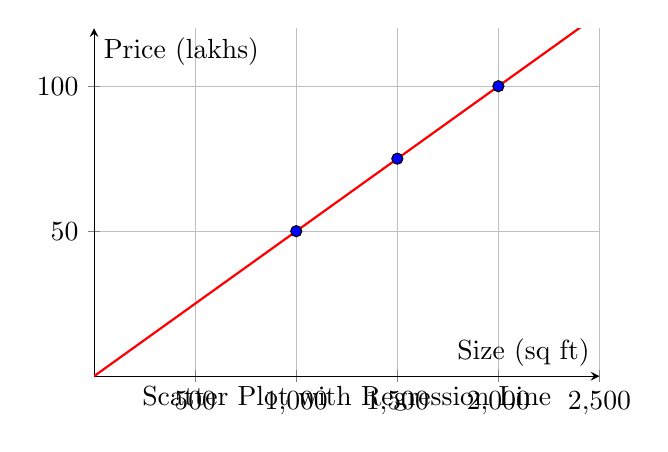
\begin{tikzpicture}
    \begin{axis}[
        xlabel={Size (sq ft)},
        ylabel={Price (lakhs)},
        xmin=0, xmax=2500,
        ymin=0, ymax=120,
        axis lines=middle,
        grid=major,
        width=8cm,
        height=6cm,
        scatter/classes={a={mark=*,draw=black,fill=blue}}
    ]
    \addplot[scatter,only marks, scatter src=explicit symbolic]
    coordinates {
        (1000, 50) [a]
        (1500, 75) [a]
        (2000, 100) [a]
    };
    \addplot[domain=0:2500, color=red, thick] {0.05*x};
    \end{axis}
    \node [below] at (current axis.south) {Scatter Plot with Regression Line};
\end{tikzpicture}
\captionof{figure}{Linear Regression Visualization}
\end{center}

\textbf{Applications:}
\begin{itemize}
    \item \textbf{Sales vs Advertising}: More ads \(\to\) More sales
    \item \textbf{Temperature vs Ice cream sales}: Hot weather \(\to\) More sales
\end{itemize}
\end{solutionbox}

\begin{mnemonicbox}
\mnemonic{One X predicts One Y with a line}
\end{mnemonicbox}

\questionmarks{4(a)}{3}{Define the following: (1)support (2) confidence.}
\begin{solutionbox}
\textbf{Support} measures how frequently an itemset appears in the dataset.

\textbf{Confidence} measures how often items in consequent appear when antecedent is present.

\begin{center}
\captionof{table}{Definitions}
\begin{tabulary}{\linewidth}{L L L}
\hline
\textbf{Measure} & \textbf{Formula} & \textbf{Example} \\
\hline
\textbf{Support} & Count(itemset)/Total transactions & Bread appears in 60\% transactions \\
\textbf{Confidence} & Support(A\(\cup\)B)/Support(A) & 80\% who buy bread also buy butter \\
\hline
\end{tabulary}
\end{center}

\textbf{Support = Frequency of occurrence} \\
\textbf{Confidence = Reliability of rule}
\end{solutionbox}

\begin{mnemonicbox}
\mnemonic{Support = How often, Confidence = How reliable}
\end{mnemonicbox}

\questionmarks{4(b)}{4}{Explain applications of unsupervised learning.}
\begin{solutionbox}
\begin{center}
\captionof{table}{Unsupervised Learning Applications}
\begin{tabulary}{\linewidth}{L L L}
\hline
\textbf{Application} & \textbf{Purpose} & \textbf{Example} \\
\hline
\textbf{Customer Segmentation} & Group similar customers & Marketing campaigns \\
\textbf{Data Compression} & Reduce data size & Image compression \\
\textbf{Anomaly Detection} & Find unusual patterns & Fraud detection \\
\textbf{Recommendation Systems} & Suggest similar items & Music recommendations \\
\hline
\end{tabulary}
\end{center}

\textbf{Customer Segmentation} groups customers with similar buying behavior for targeted marketing.

\textbf{Data Compression} reduces storage space by finding patterns and removing redundancy.

\textbf{Anomaly Detection} identifies unusual patterns that may indicate fraud or errors.
\end{solutionbox}

\begin{mnemonicbox}
\mnemonic{Segment Compress Detect Recommend}
\end{mnemonicbox}

\questionmarks{4(c)}{7}{Write and explain apriori algorithm with suitable example.}
\begin{solutionbox}
\textbf{Apriori Algorithm} finds frequent itemsets and generates association rules for market basket analysis.

\begin{center}
\captionof{table}{Algorithm Steps}
\begin{tabulary}{\linewidth}{L L L}
\hline
\textbf{Step} & \textbf{Description} & \textbf{Example} \\
\hline
\textbf{Find frequent 1-itemsets} & Count individual items & \{Bread\}:4, \{Milk\}:3 \\
\textbf{Generate 2-itemsets} & Combine frequent items & \{Bread,Milk\}:2 \\
\textbf{Apply minimum support} & Filter infrequent sets & Keep if support \(\ge\) 50\% \\
\textbf{Generate rules} & Create if-then rules & Bread \(\to\) Milk \\
\hline
\end{tabulary}
\end{center}

\textbf{Example Dataset:}
\begin{itemize}
    \item Transaction 1: \{Bread, Milk, Eggs\}
    \item Transaction 2: \{Bread, Milk\}
    \item Transaction 3: \{Bread, Eggs\}
    \item Transaction 4: \{Milk, Eggs\}
\end{itemize}

\textbf{Working Process:}
\begin{enumerate}
    \item \textbf{Scan database} to count item frequencies
    \item \textbf{Generate candidate itemsets} of increasing size
    \item \textbf{Prune infrequent itemsets} below minimum support
    \item \textbf{Generate association rules} from frequent itemsets
\end{enumerate}

\begin{center}
\begin{tikzpicture}[node distance=1.5cm, auto]
    \node [gtu block] (DB) {Transaction Database};
    \node [gtu block, right=of DB] (Freq1) {Freq 1-itemsets};
    \node [gtu block, right=of Freq1] (Gen2) {Gen 2-itemsets};
    \node [gtu block, below=1cm of Gen2] (MinSup) {Apply Min Support};
    \node [gtu block, left=of MinSup] (Rules) {Generate Rules};
    
    \path [gtu arrow] (DB) -- (Freq1);
    \path [gtu arrow] (Freq1) -- (Gen2);
    \path [gtu arrow] (Gen2) -- (MinSup);
    \path [gtu arrow] (MinSup) -- (Rules);
\end{tikzpicture}
\captionof{figure}{Apriori Algorithm Steps}
\end{center}
\end{solutionbox}

\begin{mnemonicbox}
\mnemonic{A-priori knowledge helps find frequent patterns}
\end{mnemonicbox}

\questionmarks{4(a) OR}{3}{List out the difference between clustering and classification.}
\begin{solutionbox}
\begin{center}
\captionof{table}{Clustering vs Classification}
\begin{tabulary}{\linewidth}{L L}
\hline
\textbf{Clustering} & \textbf{Classification} \\
\hline
\textbf{Unsupervised} learning & \textbf{Supervised} learning \\
No labeled data & Uses labeled training data \\
Groups similar data & Assigns predefined labels \\
\hline
\end{tabulary}
\end{center}

\textbf{Clustering} discovers hidden groups in unlabeled data.

\textbf{Classification} assigns new data to known categories using trained models.
\end{solutionbox}

\begin{mnemonicbox}
\mnemonic{Cluster = Groups unknown, Classify = Labels known}
\end{mnemonicbox}

\questionmarks{4(b) OR}{4}{Explain the clustering process in detail.}
\begin{solutionbox}
\begin{center}
\captionof{table}{Clustering Process Steps}
\begin{tabulary}{\linewidth}{L L L}
\hline
\textbf{Step} & \textbf{Description} & \textbf{Purpose} \\
\hline
\textbf{Data Preparation} & Clean and normalize data & Ensure quality input \\
\textbf{Distance Metric} & Choose similarity measure & Euclidean, Manhattan \\
\textbf{Algorithm Selection} & Pick clustering method & K-means, Hierarchical \\
\textbf{Cluster Validation} & Evaluate cluster quality & Silhouette score \\
\hline
\end{tabulary}
\end{center}

\textbf{Clustering Process} groups similar data points together based on their characteristics.

\textbf{Key decisions include choosing the number of clusters and appropriate distance metrics.}

\textbf{Validation ensures clusters are meaningful and well-separated.}
\end{solutionbox}

\begin{mnemonicbox}
\mnemonic{Prepare Distance Algorithm Validate}
\end{mnemonicbox}

\questionmarks{4(c) OR}{7}{Write and explain K-means clustering algorithm with suitable example.}
\begin{solutionbox}
\textbf{K-means} partitions data into K clusters by minimizing within-cluster sum of squares.

\begin{center}
\captionof{table}{Algorithm Steps}
\begin{tabulary}{\linewidth}{L L L}
\hline
\textbf{Step} & \textbf{Description} & \textbf{Example} \\
\hline
\textbf{Initialize centroids} & Random K center points & C1(2,3), C2(8,7) \\
\textbf{Assign points} & Each point to nearest centroid & Point(1,2) \(\to\) C1 \\
\textbf{Update centroids} & Mean of assigned points & New C1(1.5, 2.5) \\
\textbf{Repeat} & Until centroids stop moving & Convergence \\
\hline
\end{tabulary}
\end{center}

\textbf{Example: Customer Income vs Age}
\begin{itemize}
    \item Customer 1: (Income=30k, Age=25)
    \item Customer 2: (Income=35k, Age=30)
    \item Customer 3: (Income=70k, Age=45)
    \item Customer 4: (Income=75k, Age=50)
\end{itemize}

\textbf{Working Process:}
\begin{enumerate}
    \item \textbf{Choose K=2} clusters for young/old customers
    \item \textbf{Initialize centroids} randomly
    \item \textbf{Calculate distances} from each customer to centroids
    \item \textbf{Assign customers} to nearest centroid
    \item \textbf{Update centroid positions} to center of assigned customers
    \item \textbf{Repeat until stable}
\end{enumerate}

\begin{center}
\begin{tikzpicture}[node distance=1.5cm, auto]
    \node [gtu block] (K) {Choose K};
    \node [gtu block, right=of K] (Init) {Initialize Centroids};
    \node [gtu block, right=of Init] (Assign) {Assign Points};
    \node [gtu block, below=1cm of Assign] (Update) {Update Centroids};
    \node [diamond, draw, aspect=2, left=of Update] (Check) {Converged?};
    \node [gtu block, left=of Check] (Final) {Final Clusters};
    
    \path [gtu arrow] (K) -- (Init);
    \path [gtu arrow] (Init) -- (Assign);
    \path [gtu arrow] (Assign) -- (Update);
    \path [gtu arrow] (Update) -- (Check);
    \path [gtu arrow] (Check) -- node[above] {Yes} (Final);
    \path [gtu arrow] (Check.north) |- node[near start, right] {No} (Assign.south);
\end{tikzpicture}
\captionof{figure}{K-Means Logic}
\end{center}
\end{solutionbox}

\begin{mnemonicbox}
\mnemonic{K centroids Mean their assigned points}
\end{mnemonicbox}

\questionmarks{5(a)}{3}{List the applications of matplotlib.}
\begin{solutionbox}
\begin{center}
\captionof{table}{Matplotlib Applications}
\begin{tabulary}{\linewidth}{L L L}
\hline
\textbf{Application} & \textbf{Purpose} & \textbf{Example} \\
\hline
\textbf{Data Visualization} & Create charts and graphs & Bar charts, histograms \\
\textbf{Scientific Plotting} & Research presentations & Mathematical functions \\
\textbf{Dashboard Creation} & Interactive displays & Business metrics \\
\hline
\end{tabulary}
\end{center}

\textbf{Matplotlib} is Python's primary plotting library for creating static, animated, and interactive visualizations.
\end{solutionbox}

\begin{mnemonicbox}
\mnemonic{Mat-plot-lib = Math Plotting Library}
\end{mnemonicbox}

\questionmarks{5(b)}{4}{Write down code to plot a vertical line and horizontal line using matplotlib.}
\begin{solutionbox}
\begin{lstlisting}[language=Python]
import matplotlib.pyplot as plt

# Create figure
plt.figure(figsize=(8, 6))

# Plot vertical line at x=3
plt.axvline(x=3, color='red', linestyle='--', label='Vertical Line')

# Plot horizontal line at y=2
plt.axhline(y=2, color='blue', linestyle='-', label='Horizontal Line')

# Add labels and title
plt.xlabel('X-axis')
plt.ylabel('Y-axis')
plt.title('Vertical and Horizontal Lines')
plt.legend()
plt.grid(True)
plt.show()
\end{lstlisting}

\textbf{Key Functions:}
\begin{itemize}
    \item \code{axvline()}: Creates vertical line
    \item \code{axhline()}: Creates horizontal line
\end{itemize}
\end{solutionbox}

\begin{mnemonicbox}
\mnemonic{axvline = Vertical, axhline = Horizontal}
\end{mnemonicbox}

\questionmarks{5(c)}{7}{Explain features and applications of Scikit-Learn.}
\begin{solutionbox}
\begin{center}
\captionof{table}{Scikit-Learn Features}
\begin{tabulary}{\linewidth}{L L L}
\hline
\textbf{Feature} & \textbf{Description} & \textbf{Example} \\
\hline
\textbf{Simple API} & Easy to use interface & fit(), predict() \\
\textbf{Multiple Algorithms} & Various ML methods & SVM, Random Forest \\
\textbf{Data Preprocessing} & Built-in data tools & StandardScaler \\
\textbf{Model Evaluation} & Performance metrics & accuracy\_score \\
\hline
\end{tabulary}
\end{center}

\textbf{Scikit-Learn} is Python's most popular machine learning library providing simple tools for data analysis.

\textbf{Applications:}
\begin{itemize}
    \item \textbf{Classification}: Email spam detection
    \item \textbf{Regression}: House price prediction
    \item \textbf{Clustering}: Customer segmentation
    \item \textbf{Dimensionality Reduction}: Data visualization
\end{itemize}

\begin{center}
\begin{tikzpicture}[node distance=1.5cm]
    \node [gtu block] (SK) {Scikit-Learn};
    
    \node [gtu block, below left=1.5cm and 0.5cm of SK] (Class) {Classification};
    \node [gtu block, below left=1.5cm and -1.5cm of SK] (Reg) {Regression};
    \node [gtu block, below right=1.5cm and -1.5cm of SK] (Clust) {Clustering};
    \node [gtu block, below right=1.5cm and 0.5cm of SK] (Prep) {Preprocessing};
    
    \node [gtu state, below=0.8cm of Class, text width=2cm] (C_Ex) {SVM\\Trees};
    \node [gtu state, below=0.8cm of Reg, text width=2cm] (R_Ex) {Linear\\Poly};
    \node [gtu state, below=0.8cm of Clust, text width=2cm] (Cl_Ex) {K-means\\DBSCAN};
    \node [gtu state, below=0.8cm of Prep, text width=2cm] (P_Ex) {Scale\\Encode};
    
    \path [gtu arrow] (SK) -- (Class);
    \path [gtu arrow] (SK) -- (Reg);
    \path [gtu arrow] (SK) -- (Clust);
    \path [gtu arrow] (SK) -- (Prep);
    
    \path [gtu arrow] (Class) -- (C_Ex);
    \path [gtu arrow] (Reg) -- (R_Ex);
    \path [gtu arrow] (Clust) -- (Cl_Ex);
    \path [gtu arrow] (Prep) -- (P_Ex);
\end{tikzpicture}
\captionof{figure}{Scikit-Learn Components}
\end{center}
\end{solutionbox}

\begin{mnemonicbox}
\mnemonic{Scikit = Science Kit for machine learning}
\end{mnemonicbox}

\questionmarks{5(a) OR}{3}{Give the purpose of NumPy in machine learning.}
\begin{solutionbox}
\begin{center}
\captionof{table}{NumPy Purpose in ML}
\begin{tabulary}{\linewidth}{L L L}
\hline
\textbf{Purpose} & \textbf{Description} & \textbf{Benefit} \\
\hline
\textbf{Numerical Computing} & Fast array operations & Efficient calculations \\
\textbf{Foundation Library} & Base for other libraries & Pandas, Scikit-learn use it \\
\textbf{Mathematical Functions} & Built-in math operations & Statistics, linear algebra \\
\hline
\end{tabulary}
\end{center}

\textbf{NumPy} provides the foundation for numerical computing in Python machine learning applications.

\textbf{Essential for handling large datasets and performing mathematical operations efficiently.}
\end{solutionbox}

\begin{mnemonicbox}
\mnemonic{Num-Py = Numerical Python}
\end{mnemonicbox}

\questionmarks{5(b) OR}{4}{Write down steps to import csv file in pandas.}
\begin{solutionbox}
\begin{lstlisting}[language=Python]
import pandas as pd

# Step 1: Import pandas library
# Step 2: Use read_csv() function
data = pd.read_csv('filename.csv')

# Step 3: Display first few rows
print(data.head())

# Optional: Specify parameters
data = pd.read_csv('file.csv', 
                   delimiter=',',
                   header=0,
                   index_col=0)
\end{lstlisting}

\textbf{Steps:}
\begin{enumerate}
    \item \textbf{Import pandas} library
    \item \textbf{Use read\_csv()} function with filename
    \item \textbf{Verify data} with head() method
\end{enumerate}
\end{solutionbox}

\begin{mnemonicbox}
\mnemonic{Import Read Verify}
\end{mnemonicbox}

\questionmarks{5(c) OR}{7}{Explain features and applications of Pandas.}
\begin{solutionbox}
\begin{center}
\captionof{table}{Pandas Features}
\begin{tabulary}{\linewidth}{L L L}
\hline
\textbf{Feature} & \textbf{Description} & \textbf{Example} \\
\hline
\textbf{Data Structures} & DataFrame and Series & Tabular data handling \\
\textbf{Data I/O} & Read/write multiple formats & CSV, Excel, JSON \\
\textbf{Data Cleaning} & Handle missing values & dropna(), fillna() \\
\textbf{Data Analysis} & Statistical operations & groupby(), describe() \\
\hline
\end{tabulary}
\end{center}

\textbf{Pandas} is the primary data manipulation library in Python for machine learning projects.

\textbf{Key Capabilities:}
\begin{itemize}
    \item \textbf{Data Loading} from various file formats
    \item \textbf{Data Cleaning} and preprocessing operations
    \item \textbf{Data Transformation} and reshaping
    \item \textbf{Statistical Analysis} and aggregation
\end{itemize}

\begin{center}
\begin{tikzpicture}[node distance=1.5cm, auto]
    \node [gtu block] (Raw) {Raw Data};
    \node [gtu block, right=of Raw] (DF) {Pandas DataFrame};
    \node [gtu block, right=of DF] (Clean) {Cleaning};
    \node [gtu block, below=1cm of Clean] (Anal) {Data Analysis};
    \node [gtu block, left=of Anal] (Feat) {Feat Eng};
    \node [gtu block, left=of Feat] (Ready) {ML Ready Data};
    
    \path [gtu arrow] (Raw) -- (DF);
    \path [gtu arrow] (DF) -- (Clean);
    \path [gtu arrow] (Clean) -- (Anal);
    \path [gtu arrow] (Anal) -- (Feat);
    \path [gtu arrow] (Feat) -- (Ready);
\end{tikzpicture}
\captionof{figure}{Pandas Workflow}
\end{center}
\end{solutionbox}

\begin{mnemonicbox}
\mnemonic{Pandas = Panel Data for analysis}
\end{mnemonicbox}

\end{document}
